\documentclass[11pt,a4paper]{report}
\usepackage[utf8]{inputenc}
\usepackage[french]{babel}
\usepackage[T1]{fontenc}
\usepackage{amsmath}
\usepackage{amsfonts}
\usepackage{amssymb}
\usepackage{makeidx}
\usepackage{svg}
\usepackage[left=2.5cm,top=2cm,right=2.5cm]{geometry}
\author{Frantzen Christian Küpper Marius}
\title{INFO-H-303 : Base de données\\
		Projet : Annuaire d'établissements horeca}
\begin{document}
\maketitle
\section*{Modèle entité-association}

\begin{figure}[h]
  \centering
  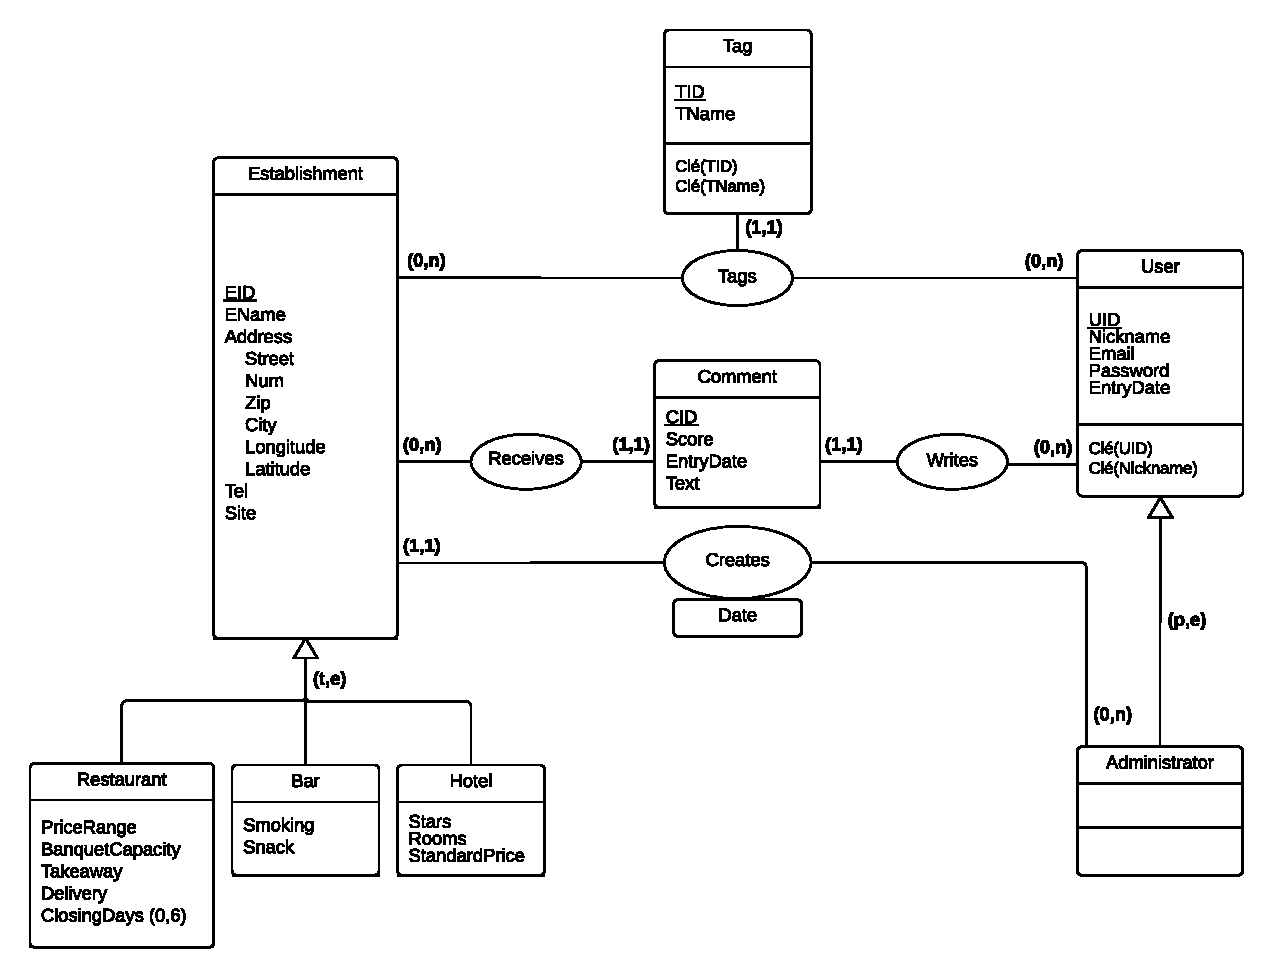
\includegraphics[width=\textwidth]{modelEA.pdf}
  \caption{Modèle entité-association}
\end{figure}


\subsection*{Contraintes d'intégrité}

\begin{itemize}
\item Un \textit{User} peut commenter plusieurs fois le même \textit{Establishment} à des dates différentes. 
\item Un \textit{User} ne peut pas apposer le même \textit{Tag} plusieurs fois sur le même \textit{Establishment}.
\item L'\textit{EntryDate} d'un \textit{Adminisitrator} doit être strictement supérieure à l'\textit{EntryDate} de l'\textit{Establishment} qu'il a créé.
\item L'\textit{EntryDate} d'un \textit{Comment} doit être strictement supérieure à l'\textit{EntryDate} du User qui le fait ainsi que l'\textit{EntryDate} de l'\textit{Establishment} sur lequel il est fait. 
\end{itemize}
\subsection*{Remarques}
Si un \textit{Restaurant} ne veut pas organiser de banquet, il spécifie sa \textit{BanquetCapacity} comme étant 0.

\section*{Modèle relationnel}
\noindent
\textbf{Establishment}(\underline{EID},EName,Street,Num,Zip,City,Longitude,Latitude,Tel,Site,UID,EntryDate)
\begin{itemize}
\item UID référence User.UID (représente le createur de l'établissement)\\
\end{itemize}
\textbf{Restaurant}(\underline{EID}, PriceRange, BanquetCapacity, Takeaway, Delivery)
\begin{itemize}
\item EID référence Establishment.EID\\
\end{itemize} 
\textbf{RestaurantClosingDays}(\underline{EID}, ClosingDay, Hour)
\begin{itemize}
\item EID référence Establishment.EID\\
\end{itemize}
\textbf{Bar}(\underline{EID}, Smoking, Snack)
\begin{itemize}
\item EID référence Establishment.EID\\
\end{itemize}
\textbf{Hotel}(\underline{EID}, Stars, Rooms, StandardPrice)
\begin{itemize}
\item EID référence Establishment.EID\\
\end{itemize}
\textbf{User}(\underline{UID}, Nickname, Email, Password, EntryDate, Admin)
\begin{itemize}
\item Nickname est unique et donc également une clé de cette relation
\item Email est unique et donc également une clé de cette relation\\
\end{itemize}
\textbf{Comment}(\underline{CID}, UID, EID, EntryDate, Score,  Text)
\begin{itemize}
\item UID référence User.UID
\item EID référence Establishment.EID
\item (UID,EID,EntryDate) est unique et donc également une clé de cette relation\\
\end{itemize}
\textbf{Tag}(\underline{TID}, TName)
\begin{itemize}
\item TName est unique et donc également une clé de cette relation\\
\end{itemize}
\textbf{EstablishmentTag}(\underline{TID, EID, UID})
\begin{itemize}
\item TID référence Tag.TID
\item EID référence Establishment.EID
\item UID référence User.UID
\end{itemize}
\subsection*{Remarques}
L'ajout d'une entrée dans \textit{Establishment} implique l'ajout d'une entrée dans soit \textit{Restaurant}, soit \textit{Bar} ou soit \textit{Hotel}. Les deux entrées ont le même \textit{EID}.
\subsection*{Contraintes de domaine}
\begin{itemize}
\item $User.Admin \in \{True,False\} $ (Seul les \textit{User} avec \textit{User.Admin} = True ont les droits de créer, supprimer ou modifier des \textit{Establishment}).
\item Pour les entrées dans \textit{Comment}, \textit{Comment.EntryDate > Establishment.EntryDate} et \textit{Comment.EntryDate} > \textit{User.EntryDate}
\item $Comment.Score \in \{0,1,2,3,4,5\}$
\item $Hotel.Stars \in \{0,1,2,3,4,5\}$
\item $Hotel.Rooms \in \mathbb{N}_{0}$
\item $Hotel.StandardPrice \in \mathbb{R}^{+}_{0}$
\item $Restaurant.BanquetCapacity \in \mathbb{N} $
\item $Restaurant.PriceRange \in \mathbb{R}^{+}_{0} $
\item $Restaurant.Takeaway \in \{True,False\} $
\item $Restaurant.Delivery \in \{True,False\} $
\item $RestaurantClosingDays.Hour \in \{"AM","PM"\}$ (matin / après-midi)
\item $RestaurantClosingDays.ClosingDay \in \{0,1,2,3,4,5,6\}$
\item $Bar.Smoking \in \{True,False\} $
\item $Bar.Snack \in \{True,False\} $
\end{itemize}


\section*{Hypothèses}
\noindent

\begin{itemize}
\item \underline{Deux \textit{User}s ne peuvent pas avoir le même \textit{Nickname}:} L'interface doit permettre de consulter la fiche de chaque \textit{User}. Un \textit{User} qui cherche le profil de quelqu'un ne peut pas distinguer deux \textit{User}s avec le même \textit{Nickname} puisque le celui-ci est la seule donnée visible (pas d'image de profil, etc ...).
\item \underline{Un \textit{Admin} ne peut pas modifier des \textit{Comment}s ni des \textit{Tag}s:} On pourrait lui donner les droits de gestion pour vérifier qu'il n'y ait pas d'abus, mais pour le moment un \textit{Admin} ne peut que créer, modifier et enlever des \textit{Establishment}s.
\end{itemize}

\section*{Requêtes}
\subsection*{R1}
\noindent Tous les utilisateurs qui apprécient au moins 3 établissements que l'utilisateur "Brenda" apprécie.
\paragraph*{Calcul relationnel tuple}
\begin{align*}
\{ u | User(u) & \wedge \exists e_{1} \exists e_{2} \exists e_{3} ( Establishment(e_{1}) \wedge
Establishment(e_{2}) \wedge Establishment(e_{3}) \wedge \\ 
& e_{1} \neq e_{2} \wedge e_{1} \neq e_{3} \wedge e_{2} \neq e_{3} \wedge \exists u_{2} \exists c_{1} \exists c_{2} ( User(u_{2}) \wedge Comment(c_{1}) \wedge Comment(c_{2}) \wedge \\
& u_{2}.nickname = "Brenda" \wedge \forall i \in \{1,2,3 \}(c_{1}.uid=e_{i} \wedge c_{2}.uid=e_{i} \wedge c_{1}.uid = u.uid \wedge \\
&  c_{2}.uid = u_{2}.uid \wedge  c_{1}.score \geq 4 \wedge  c_{2}.score \geq 4  )))
\}
\end{align*}
\paragraph*{algèbre relationnelle}
\subsection*{R2}
\noindent Tous les établissements qu’apprécie au moins un utilisateur qui apprécie tous les établissements que "Brenda" apprécie.
\paragraph*{Calcul relationnel tuple}
\begin{align*}
s
\end{align*}
\paragraph*{algèbre relationnelle}
\subsection*{R3}
Tous les établissements pour lesquels il y a au plus un commentaire.
\paragraph*{Calcul relationnel tuple}
\begin{align*}
s
\end{align*}
\paragraph*{algèbre relationnelle}
\subsection*{R4}
La liste des administrateurs n’ayant pas commenté tous les établissements qu’ils ont crées.
\paragraph*{Calcul relationnel tuple}
\begin{align*}
s
\end{align*}
\paragraph*{algèbre relationnelle}

\end{document}